\chapter{Package xkcd: Plotting ggplot2 graphics in a XKCD style}

\chapterprecis{Emilio Torres Manzanera\\Universidad de Oviedo}

\index{Torres Manzanera, Emilio}

\index[inst]{Universidad de Oviedo}

Se presenta el paquete xkcd, que realiza gráficos ggplot2 como si fueran trazados a mano, siguiendo el estilo de las tiras cómicas de XKCD.

 \bigskip \begin{center} 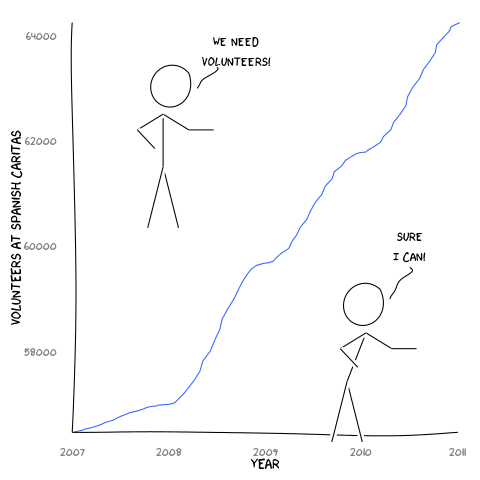
\includegraphics[width=.33\textwidth]{Logos/caritas.png} 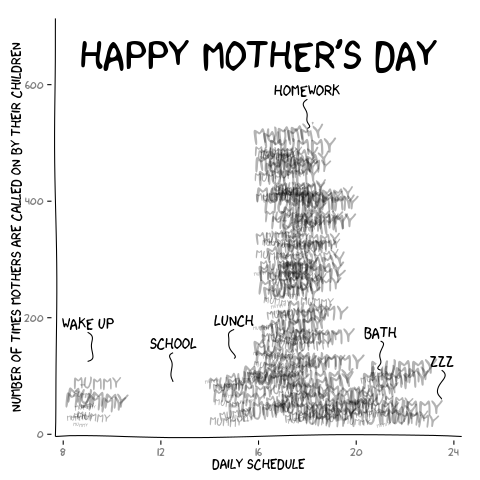
\includegraphics[width=.33\textwidth]{Logos/mothersday.png} \end{center}

%\bibliographystyle{plain}

%\bibliography{resumenes/package_xkcd__plotting_ggplot2_graphics_in_a_xkcd_style}
